% Exponents in 10! = 2^8 * 3^4 * 5^2 * 7.
% Layers are floor(10/p), floor(10/p^2), floor(10/p^3): (5,2,1), (3,1), (2), (1).
% One exponent unit is 0.48 on the vertical axis.
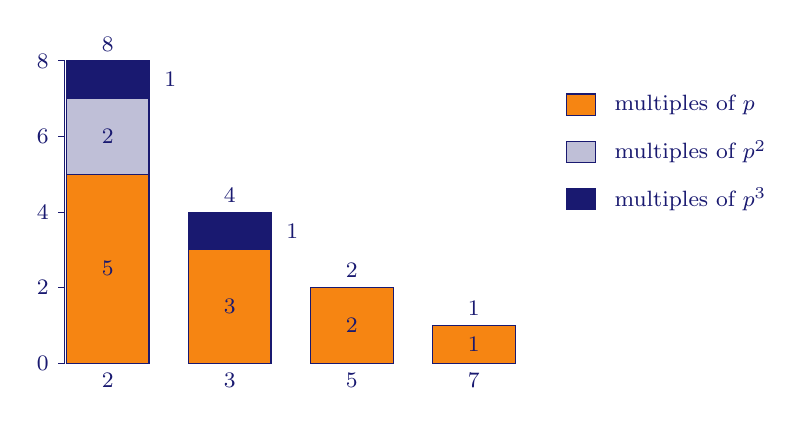
\begin{tikzpicture}[every node/.style={font=\footnotesize}]
  % p = 2, layers 5 + 2 + 1
  \fill[BurntOrange] (0,0) rectangle (1.05,2.40);
  \fill[MidnightBlue!28] (0,2.40) rectangle (1.05,3.36);
  \fill[MidnightBlue] (0,3.36) rectangle (1.05,3.84);
  \draw[MidnightBlue] (0,0) rectangle (1.05,3.84);
  \draw[MidnightBlue] (0,2.40)--(1.05,2.40);
  \draw[MidnightBlue] (0,3.36)--(1.05,3.36);
  \node[MidnightBlue] at (0.525,1.20) {$5$};
  \node[MidnightBlue] at (0.525,2.88) {$2$};
  \node[MidnightBlue,anchor=west] at (1.12,3.60) {$1$};
  \node[MidnightBlue,below] at (0.525,0) {$2$};
  \node[MidnightBlue,above] at (0.525,3.84) {$8$};
  % p = 3, layers 3 + 1
  \fill[BurntOrange] (1.55,0) rectangle (2.60,1.44);
  \fill[MidnightBlue] (1.55,1.44) rectangle (2.60,1.92);
  \draw[MidnightBlue] (1.55,0) rectangle (2.60,1.92);
  \draw[MidnightBlue] (1.55,1.44)--(2.60,1.44);
  \node[MidnightBlue] at (2.075,0.72) {$3$};
  \node[MidnightBlue,anchor=west] at (2.67,1.68) {$1$};
  \node[MidnightBlue,below] at (2.075,0) {$3$};
  \node[MidnightBlue,above] at (2.075,1.92) {$4$};
  % p = 5, layer 2
  \fill[BurntOrange] (3.10,0) rectangle (4.15,0.96);
  \draw[MidnightBlue] (3.10,0) rectangle (4.15,0.96);
  \node[MidnightBlue] at (3.625,0.48) {$2$};
  \node[MidnightBlue,below] at (3.625,0) {$5$};
  \node[MidnightBlue,above] at (3.625,0.96) {$2$};
  % p = 7, layer 1
  \fill[BurntOrange] (4.65,0) rectangle (5.70,0.48);
  \draw[MidnightBlue] (4.65,0) rectangle (5.70,0.48);
  \node[MidnightBlue] at (5.175,0.24) {$1$};
  \node[MidnightBlue,below] at (5.175,0) {$7$};
  \node[MidnightBlue,above] at (5.175,0.48) {$1$};
  % scale
  \draw[MidnightBlue] (-0.02,0)--(-0.02,3.84);
  \draw[MidnightBlue] (-0.02,0)--(-0.10,0) node[left] {$0$};
  \draw[MidnightBlue] (-0.02,0.96)--(-0.10,0.96) node[left] {$2$};
  \draw[MidnightBlue] (-0.02,1.92)--(-0.10,1.92) node[left] {$4$};
  \draw[MidnightBlue] (-0.02,2.88)--(-0.10,2.88) node[left] {$6$};
  \draw[MidnightBlue] (-0.02,3.84)--(-0.10,3.84) node[left] {$8$};
  % legend, in the empty region to the right of the short bars
  \fill[BurntOrange] (6.35,3.15) rectangle (6.72,3.42);
  \draw[MidnightBlue] (6.35,3.15) rectangle (6.72,3.42);
  \node[MidnightBlue,anchor=west] at (6.84,3.285) {multiples of $p$};
  \fill[MidnightBlue!28] (6.35,2.55) rectangle (6.72,2.82);
  \draw[MidnightBlue] (6.35,2.55) rectangle (6.72,2.82);
  \node[MidnightBlue,anchor=west] at (6.84,2.685) {multiples of $p^2$};
  \fill[MidnightBlue] (6.35,1.95) rectangle (6.72,2.22);
  \draw[MidnightBlue] (6.35,1.95) rectangle (6.72,2.22);
  \node[MidnightBlue,anchor=west] at (6.84,2.085) {multiples of $p^3$};
\end{tikzpicture}
